\begin{frame}
 \frametitle{Rotational Effect}

 \begin{itemize}
  \item Rigid rod $OP$, fixed at $O$, $\textbf{r}=\textbf{OP}$. Force $\textbf{F}$ applied at $P$.
 \end{itemize}
%
\begin{figure}[h]
  \psfrag{F}{$\textbf{F}$}
  \psfrag{r}{$\textbf{r}$}
  \psfrag{O}{$O$}
  \psfrag{P}{$P$}
  \psfrag{}{$\alpha$}
  \psfrag{pfr}{$\textbf{proj}_{\bm{r}} \textbf{F}$}
  \psfrag{ofr}{$\textbf{orth}_{\bm{r}} \textbf{F}$}
  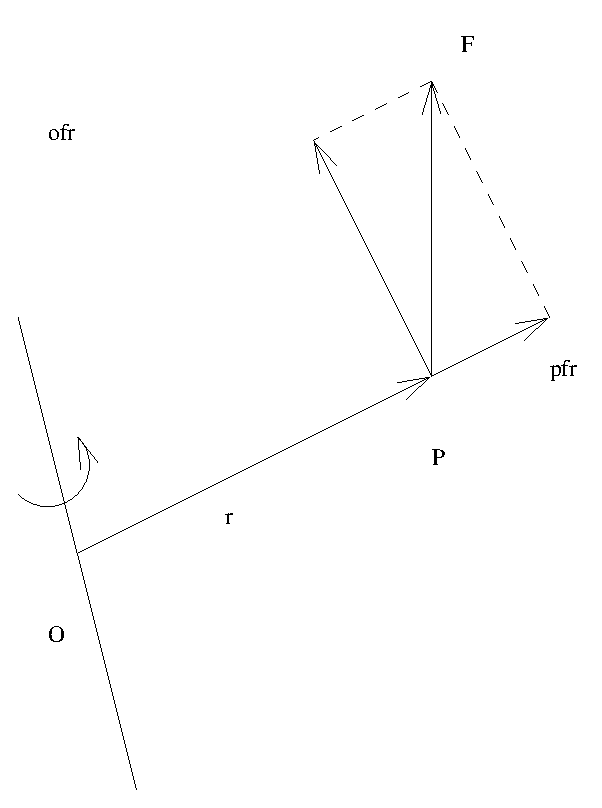
\includegraphics[height=1.5in]{../../modules/vectors/pictures/ok-torque.eps}
\end{figure}
%
\pause
\begin{itemize}
  \item $\textbf{proj}_{\bm{r}} \textbf{F}$: \pause no effect;
  \item $\textbf{orth}_{\bm{r}} \textbf{F}$: \pause rotational effect:\pause
  \begin{itemize}
    \item Axis of rotation: \pause perpendicular to $\textbf{r}$ and $\textbf{F}$;\pause
    \item Angular velocity: \pause proportional to $|\textbf{orth}_{\bm{r}} \textbf{F}|$;\pause
    \item Linear velocity: \pause proportional to $|\textbf{r}| \, |\textbf{orth}_{\bm{r}} \textbf{F}|$.
  \end{itemize}
\end{itemize}

\end{frame}